\documentclass[tikz]{standalone}
\usetikzlibrary{shapes.geometric, positioning}
\begin{document}
\tiny
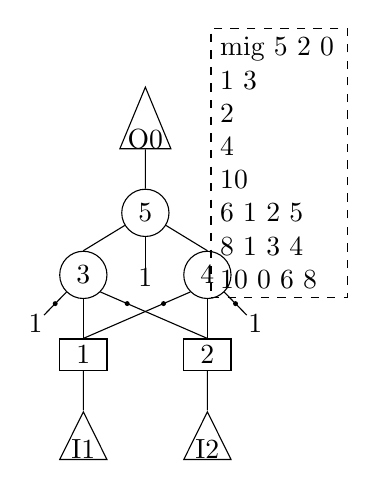
\begin{tikzpicture}[
    node distance = .5cm,
    io/.style={
        draw, isosceles triangle, isosceles triangle stretches, shape border rotate=90,
        inner sep=0pt, minimum width=.6cm, minimum height=.5cm
    },
    maj/.style={
        draw, circle, inner sep=0pt, minimum size=.6cm
    },
    pi/.style={
        draw, rectangle, inner sep=0pt, minimum width=.6cm, minimum height=.4cm,
    },
    circ/.style={
        fill, circle, inner sep=0pt, minimum size=1.8pt,
    },
    zero/.style={
        inner sep=0pt, minimum width=.2cm, minimum height=.2cm,
    }
]

    \node[io](o0){O0};
    \node[maj,below=of o0](m1){5};
    \node[maj,below left=of m1](m2){3};
    \node[maj,below right=of m1](m3){4};
    \node[pi,below=of m2](p1){1};
    \node[pi,below=of m3](p2){2};
    \node[io,below=of p1](i1){I1};
    \node[io,below=of p2](i2){I2};

    \node[zero,below=.4 of m1](z1){1};
    \node[zero,below left=.4 of m2](z2){1};
    \node[zero,below right=.4 of m3](z3){1};

    \draw (o0) to (m1);
    \draw (m1) to (m2.north);
    \draw (m1) to (m3.north);
    \draw (m2.south east) to node[circ,near start]{}(p2.north);
    \draw (m3.south west) to node[circ,near start]{}(p1.north);
    \draw (m2) to (p1.north);
    \draw (m3) to (p2.north);
    \draw (p1) to (i1);
    \draw (p2) to (i2);

    \draw (m1) to (z1);
    \draw (m2) to node[circ]{}(z2);
    \draw (m3) to node[circ]{}(z3);


    \node[text width=1.5cm, draw, rectangle, dashed] at (1.7,-.3) {
        mig 5 2 0 1 3\\
        2\\
        4\\
        10\\
        6 1 2 5\\
        8 1 3 4\\
        10 0 6 8
    };

\end{tikzpicture}
\end{document}
